\chapter{Normas y Producto Interno}
\setcounter{equation}{0}

\section{Normas en $\K^n$}

La distancia del punto $(x,y)\in \R^2$  al origen puede calcularse por el teorema de Pitágoras
$$
z = \sqrt{x^2 + y^2}.
$$
Generalizando esa fórmula a espacios de cualquier dimensión, definimos una norma vectorial:
$$
\|\vb\|_2 = \sqrt{v_1^2 + \dots + v_n^2},
$$
Esta norma suele llamarse norma-$2$ o norma euclídea. Esta norma,  a su vez, puede escribirse equivalentemente como
$$
\|\vb\|_2 = \sqrt{|v_1|^2 + \dots + |v_n|^2},
$$
lo cual nos da una expresión aplicable a los complejos.

\tccdefi
\begin{defi}
Una norma de un $K$-espacio vectorial es una función $\| \cdot \| : V \rightarrow \R_{\ge 0}$ que cumple las siguientes propiedades:
\begin{enumerate}
\item $\|a \vb\| = |a| \|\vb\|$, para $a \in \K$ y $\vb \in V$.
\item Si $\|\vb\| = 0$, entonces $\vb = 0$.
\item $\|\ub + \vb\| \le \|\ub\| + \|\vb\|$, para todo $\ub, \vb \in V$ \qquad (desigualdad triangular)
\end{enumerate}
\end{defi}
\etcc
Es fácil ver que la norma-2 cumple las primeras dos propiedades.  La tercera propiedad puede probarse usando la siguiente desigualdad clásica.

\begin{prop}[Desigualdad de Cauchy-Schwarz]
\label{prop:CS}
Dados $\ub, \vb \in \K^n$,
$$
\left|\sum_{i=1}^{n} \overline u_{i}v_{i}\right|\leq \|\ub\|_2\|\vb\|_2.
$$
\end{prop}
\begin{proof}
Asumamos primero que $\K=\R$. Consideremos el siguiente polinomio de grado 2 en la variable $x$
$$
p(x) = (u_1 x + v_1)^2 + \dots + (u_n x +v_n)^2  =\left(\sum _{i=1}^nu_{i}^{2}\right)x^{2}+2\left(\sum _{i=1}^nu_{i}v_{i}\right)x+\sum _{i=1}^nv_{i}^{2}.
$$

Como $p$ es una suma de cuadrados, $p(x) \ge 0$ para todo $x \in \R$  tiene o bien un raiz real doble o raíces complejas. Escribiendo $p(x)=ax^2 + bx + c$ vemos que debe ser entonces $b^2-4ac \le 0$. Es decir,
$$
4 \left(\sum _{i}u_{i}v_{i}\right)^{2}- 4 \left(\sum _{i}{u_{i}^{2}}\right)\left(\sum _{i}{v_{i}^{2}}\right)\leq 0,
$$
y eliminando el factor 4 y despejando, obtenemos la desigualdad buscada.

Si $\K=\C$ notamos, por la desigualdad triangular en los complejos\footnote{Si escribimos $z_1=a_1+ib_1,z_2=a_2+ib_2\in \C$, resulta
$|z_1+z_2|\le|z_1|+|z_2|$ sí y solo sí
$$(a_1+a_2)^2+(b_1+b_2)^2\le \left(\sqrt{a_1^2+b_1^2}+\sqrt{a_2^2+b_2^2}\right)^2,$$ desarrollar el cuadrado y ver que eso ocurre sí y solo sí $0\le(a_1b_2-a_2b_1)^2$ que obviamente siempre es válido.}


$$
\left|\sum _{i}u_{i}\overline{v_{i}}\right|\le \sum _{i}|u_{i}||\overline{v_{i}}|=\sum _{i}|u_{i}||{v_{i}}|,
$$
y la desigualdad sale ahora usando el caso real con los vectores $(|u_1|,\cdots,|u_n|)$,$(|v_1|,\cdots,|v_n|)$.
\end{proof}
\begin{rem}
Notar que la desigualdad de Cauchy-Schwarz vale también tomando a la izquierda
$\sum _{i}\overline{u_{i}}{v_{i}}$, puesto que $\sum _{i}\overline{u_{i}}{v_{i}}=\overline{\sum _{i}u_{i}\overline{v_{i}}}$ y el módulo de un complejo es igual al de su conjugado.
\end{rem}
\begin{cor}
 Para todo $\ub,\vb\in \K^n$ vale,
 $\|\ub+\vb\|_2\le\|\ub\|_2+\|\vb\|_2.$
\end{cor}
\begin{proof}
La hacemos en $\C$ y en $\R$  sale como caso particular.
$$
\|\ub+\vb\|_2^2=
\sum_{i=1}^n |u_i+v_i|^2=\sum_{i=1}^n (u_i+v_i)\overline{(u_i+v_i)}
$$
$$
=\sum_{i=1}^n u_i\overline{u_i}+
\sum_{i=1}^n(u_i\overline{v_i}+v_i\overline{u_i})+\sum_{i=1}^n v_i\overline{v_i}=\|\ub\|_2^2+\sum_{i=1}^n(u_i\overline{v_i}+v_i\overline{u_i})+\|\vb\|^2_2,
$$
los términos entre paréntesis son reales (un número complejo -eventualmente complejo- mas su conjugado), luego
$$
\sum_{i=1}^n(u_i\overline{v_i}+v_i\overline{u_i})\le
\left|\sum_{i=1}^n(u_i\overline{v_i}+v_i\overline{u_i})\right|\le\left|\sum_{i=1}^nu_i\overline{v_i}\right|+\left|\sum_{i=1}^nv_i\overline{u_i}\right| \le 2\|\ub\|_2\|\vb\|_2,
$$
donde hemos usado Cauchy-Schwarz en la última desigualdad.
Luego, se tiene
$$
\|\ub+\vb\|_2^2\le \|\ub\|^2+\|\vb\|^2+2\|\ub\|_2\|\vb\|_2=
\left(\|\ub\|_2+\|\vb\|_2\right)^2,
$$
lo que termina la demostración tomando raíz cuadrada \end{proof}
\tccdefi
Como generalización de la norma$-2$, están las normas$-p$, definidas también en  $\K^{n}$:

\begin{itemize}
\item Norma$-1$: $\| \vb \|_1 = |v_1| + \dots + |v_n|$
\item Norma-infinito: $\| \vb \|_\infty = \max\{|v_1|, \dots, |v_n|\}$
\item Norma$-p$: $\| \vb \|_p = \left(|v_1|^p  + \dots + |v_n|^p \right)^{1/p}$
\end{itemize}
\etcc

En el siguiente gr\'afico podemos ver la diferencia entre las 3 normas m\'as usuales en $\R^2$. En cada gr\'afico est\'an representados todos los puntos con norma igual a 1 bajo la norma respectiva.
\clearpage
\begin{figure}
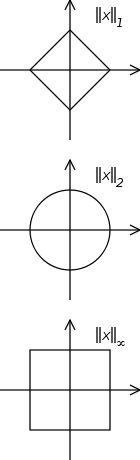
\includegraphics[scale=.3]{140px-Vector_norms.png}
\caption{``Círculos''  de radio 1 en diferentes normas. Es decir $\vb\in \R^2$ tales que $\|\vb\|=1$.}
\end{figure}
En la siguiente figura observamos distintas curvas de nivel\footnote{Las curvas en las cuales la norma respectiva permanece constante.} para distintas normas.
\begin{ej}
 Examinando los gráficos de las curvas de
nivel de las normas$-p$ se puede intuir que  $\lim_{p\to +\infty}\|\vb\|_p=\|\vb\|_\infty$. De una demostración de este hecho.
\end{ej}
\begin{figure}
 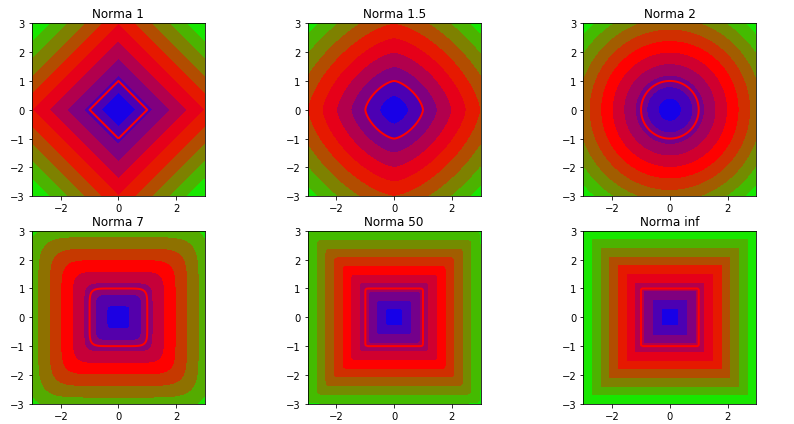
\includegraphics[scale=.4]{nivelNormas.png}
\caption{Curvas de nivel de diferentes normas$-p$.}
\end{figure}
% \begin{aplicacion}
% Para entender la diferencia entre las distintas normas, analizamos el siguiente ejercicio: Hallar gr\'aficamente el punto del plano de norma igual a 1 que maximiza la funci\'on $f(x,y) = 2y + x$. Para resolverlo, graficamos en el plano todos los puntos para los cuales $f$ tiene un valor fijo. Por ejemplo, los puntos para los cuales $f(x,y) = 3$ se encuentran en una recta que pasa por el punto $(3,0)$ y tiene pendiente $-1/2$. Si aumentamos o disminuimos este valor fijo, obtendremos una recta paralela a la anterior desplazada hacia la derecha o izquierda respectivamente.
%
% Por lo tanto, para resolver el problema, desplazamos la recta que trazamos hacia la izquierda hasta que toque a alguno de los puntos de norma 1.
% Concluimos que en el caso de la norma-1 este punto es el punto $(1,0)$, para la norma infinito este punto es el punto $(1,1)$ y para la norma 2, este punto es un punto en el arco del primer cuadrante.
%
% En general, al maximizar o minimizar la norma-1 de una función, obtendremos puntos con varias coordenadas nulas, mientras que al minimazar la norma-2 encontraremos puntos con coordenadas no nulas de valor menor que las de la norma-1. Dependiendo la aplicación resultará m\'as \'util una u otra de las normas.
% \end{aplicacion}
Para nosotros va a ser relevante medir \emph{errores} en espacios vectoriales, para ello recordemos que dados $\ub,\vb\in \R^n$
$\|\ub-\vb\|_2$ da la distancia entre ellos. En ocasiones, sin embargo, vamos a notar que es mas sencillo trabajar con una norma diferente a la norma-$2$, por lo que resulta natural ver que relación hay entre las diferentes normas-$p$. Puede probarse muy fácilmente lo siguiente.
\begin{ej}
Verificar que para todo $\xb\in \K^n$
\begin{enumerate}
\item $\|\xb\|_2 \le \|\xb\|_1 \le \sqrt{n} \|\xb\|_2$
\item $\|\xb\|_\infty \le \|\xb\|_2 \le \sqrt{n} \|\xb\|_\infty$
\item $\|\xb\|_\infty \le \|\xb\|_1 \le n \|\xb\|_\infty$
\end{enumerate}
\end{ej}
Ese resultado es un caso particular de uno mucho mas general. Primero definamos \emph{equivalencia de normas}.
\tccdefi
\begin{defi}
 Sean $\|\cdot\|$ y $\|\cdot\|_{*}$ dos normas en un $\K$-espacio vectorial $V$. Decimos que son equivalentes si existen dos constantes $0<c,C$ tales que para todo $\xb\in V$
 $$
 c\|\xb\|_* \le \|\xb\| \le C \|\xb\|_*
 $$
\end{defi}
\etcc
Vale lo siguiente,
\begin{prop}
\label{prop:equivnorm}
 En un $\K$-espacio vectorial de dimensión finita todas la normas son equivalentes\footnote{Las constantes que relacionan las normas dependen de la dimensión $n$, típicamente se deterioran si $n\to \infty$}.
\end{prop}
Este resultado nos es útil en muchos contextos.  Veamos primero la siguiente definición.
\tccdefi
\begin{defi}
Decimos que una sucesi\'on de vectores $\{v_n\}_{n \in \N}$ converge bajo una norma $\|\cdot\|$ a un vector $v$ si
$$
\|v_n - v\| \rightarrow 0 \quad \text{ cuando } n \rightarrow \infty.
$$
\end{defi}
\etcc
Como consecuencia de la Proposición \ref{prop:equivnorm}, la convergencia en una norma cualquiera implica la convergencia en todas las normas.

\section{Producto Interno}
\tccdefi
\begin{defi}
Dados dos vectores $\ub, \vb \in \K^n$ definimos\footnote{Recordemos que asociamos los vectores con las matrices columna.} el producto interno (canónico) por la fórmula\footnote{En muchos casos se suele conjugar los coeficientes del $\vb$ en la sumatoria en vez de los de $\ub$  en la definición de $\langle \ub,\vb\rangle$. Para nuestros intereses no cambia en absoluto la definición utilizada que por lo demas coinciden sobre $\R$.} $$
\langle \ub, \vb \rangle = \ub^*\vb\in \K,
$$
es decir
$$
\langle \ub, \vb \rangle=\overline{u_1} v_1 + \overline{u_2} v_2 + \dots + \overline{u_n} v_n = \sum_{i=1}^{n} \overline{u_i}v_i.
$$
\end{defi}
\etcc
Tenemos las siguientes propiedades inmediatas.

\tcc
\begin{rem}
\label{obs:interno}
Notar que para $\xb,\yb,\zb \in \K^n$, $\wb\in \K^m$ $a,b \in \K$,  $\Ab\in \K^{n \times m}$, resulta

\begin{enumerate}
\item   $\langle \xb, \yb \rangle= \overline{\langle \yb, \xb \rangle}$,
\item   $\langle \xb, a\yb + b\zb \rangle = a \langle \xb, \yb \rangle + b \langle \xb, \zb \rangle$,  y $\langle a\yb + b\zb,\xb \rangle = \overline{a} \langle \yb, \xb \rangle + \overline{b} \langle \zb, \xb \rangle$.
\item  $\langle \Ab\wb, \xb \rangle = \langle  \wb,\Ab^* \xb \rangle$\footnote{Puesto que $\langle \Ab\wb, \xb \rangle = (\Ab\wb)^*\xb=\wb^*\Ab^*\xb= \langle  \wb,\Ab^* \xb \rangle$.}
  \item $\langle a\xb, a\yb \rangle = \overline{a}a \langle \xb, \yb \rangle=|a|^2 \langle \xb, \yb \rangle$.
\item  Utilizando el producto interno, la norma-$2$ de un vector se puede definir por la fórmula $\|\vb\| = \sqrt{\langle \vb, \vb\rangle}$.
\item La desigualdad de Cauchy-Schwarz se escribe
$|\langle \vb,\wb\rangle|\le \|\vb\|_2\|\wb\|_2,$
 \end{enumerate}
\end{rem}
\etcc

\begin{ejemplo}
$\langle \xb + \yb, \xb + \yb\rangle = \langle \xb, \xb + \yb\rangle + \langle \yb, \xb + \yb\rangle = \langle \xb, \xb \rangle + \langle \xb, \yb \rangle + \langle \yb, \xb \rangle + \langle \yb, \yb\rangle = \|\xb\|^2 + 2\langle \xb, \yb \rangle + \|\yb\|^2$
\end{ejemplo}
Sean $\xb,\yb\in \R^2$, $\xb\neq \cero\neq \yb$, $\xb=(a_1,a_2)$, $\yb=(b_1,b_2)$.   Podemos escribir $\xb=\|\xb\|\frac{\xb}{\|\xb\|}$ y como $ \frac{\xb}{\|\xb\|}$ está en el círculo de radio $1$ vemos que existe un único $\alpha$, $0\le \alpha<2\pi$ tal que
$ \frac{\xb}{\|\xb\|}=(\cos(\alpha),\sen(\alpha))$. Es decir, $\xb=\|\xb\|_2(\cos(\alpha),\sen(\alpha))$. Análogamente, podemos escribir $\yb=\|\yb\|_2(\cos(\beta),\sin(\beta))$ y en particular\footnote{Recordar: $
cos(\alpha +\beta)=cos(\alpha)cos(\beta)-sen(\alpha)sen(\beta),
$
$
sen(\alpha +\beta)=sen(\alpha)cos(\beta)+cos(\alpha)sen(\beta).
$
}
$$
\langle \xb,\yb\rangle= \|\xb\|_2\|\yb\|_2\left(\cos(\alpha)\cos(\beta)+\sen(\alpha)\sen(\beta)\right)=\|\vb\|_2\|\wb\|_2\cos(\alpha-\beta),
$$
lo que dice que puede escribirse
\begin{equation}
 \label{eq:calculodeAng}
\cos(\theta)=\frac{\langle \xb,\yb\rangle}{\|\vb\|_2\|\wb\|_2},
\end{equation}
con $\theta$ el ángulo\footnote{Considerando que $\cos(\mu)=\cos(2\pi-\mu)$ siempre puede elegirse $0\le \theta < \pi$.} entre $\xb$ y $\yb$.
\begin{center}
 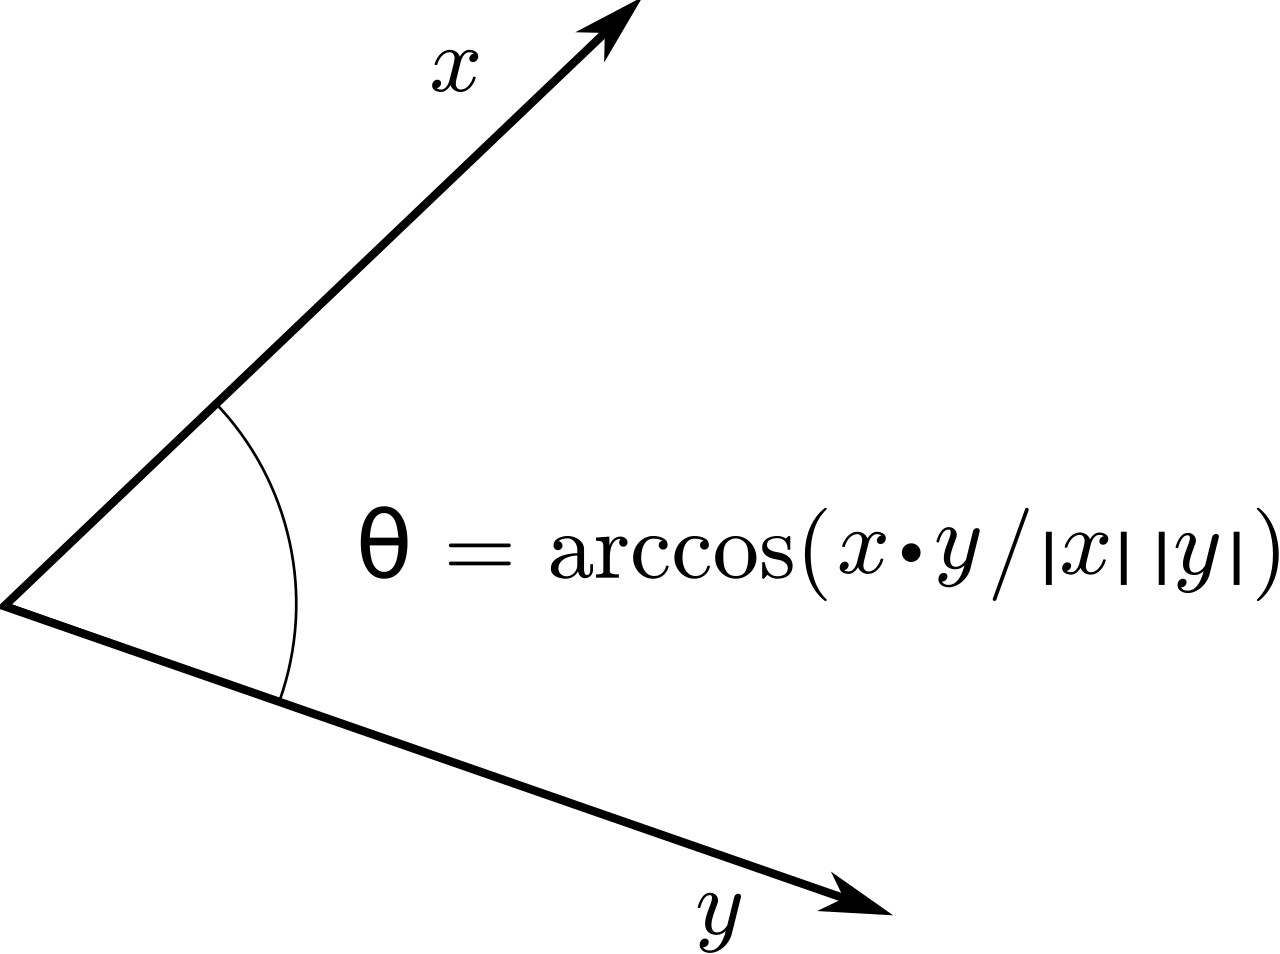
\includegraphics[scale=0.1]{angulo.png}
\end{center}
En $\Rn$ ocurre lo mismo. Ya que $-1\le\frac{\langle \xb, \yb\rangle}{\|\xb\|\|\yb\|}\le 1$, (ver (6) de la Observación \ref{obs:interno}) se define el ángulo $\theta$ entre $\xb$ e $\yb$ a través de \eqref{eq:calculodeAng}.



\tcc
Las normas nos han permitido incorporar al \emph{álgebra} (el espacio vectorial) el concepto de distancia, que  nos permitirá introducir la noción de convergencia y una forma de medir errores.  El producto escalar, por su parte, nos permite trabajar con ángulos. En particular con la idea de perpendicularidad u ortogonalidad que resulta  fundamental en el desarrollo de algoritmos estables.
\etcc
De \eqref{eq:calculodeAng} vemos que $\theta=\pi/2$ si y solo si $\vb^*\wb=0$, de ahí la siguiente definición que la extendemos a los complejos.
\tccdefi
\begin{defi}
 Dados $\vb,\wb\in\K^n$, no nulos. Decimos que son ortogonales sí y solo sí  $\vb^*\wb=\langle \vb,\wb\rangle=0.$ En este caso también usaremos la notación $\vb\perp \wb$.
\end{defi}
\etcc
\tccdefi
\begin{defi}
 Una colección de vectores  $\{\vb_i\}_{1\le i\le k}\subset \K^{n}$ se dice \emph{ortogonal} si $\langle \vb_i,\vb_j\rangle =\delta_i^j$. Si además $\|\vb_i\|_2=1$ para todo $1\le i\le k$ decimos que el conjunto es \emph{ortonormal.}
\end{defi}
\etcc
Los conjuntos ortogonales tienen muchas propiedades que pueden explotarse, tanto teóricamente como en la práctica.

Veamos una de ellas de importancia fundamental. Sea $\mathcal{B}=\{\vb\}_{1\le i\le n}\subset \K^n$ una \emph{base} ortonormal de $\K^n$. Dado $\wb\in \K^n$ queremos conocer las coordenadas de $\wb$ en la base $\mathcal{B}$. Esto se reduce a hallar los  $\{\alpha_i\}_{1\le i\le n}\subset \K$ tales que
\begin{equation}
\label{eq:escritura_ort}
\wb=\sum_{i=1}^n\alpha_i\vb_i,
\end{equation}
que como sabemos implica resolver un sistema de $n\times n$. Sin embargo en este caso particular, vemos que para cada $1\le j\le n$ el producto escalar
\begin{equation}
\label{eq:proyecciones}
\vb_j^*\wb=\sum_{i=1}^n\alpha_i\vb_j^*\vb_i=\alpha_j,
\end{equation}
permite ``despejar'' $\alpha_i$ por el módico costo de un producto escalar\footnote{Esto es $2n-1$ operaciones, $n$ productos y $n-1$ sumas.}
Desde el punto de vista matricial, sea $\Qb\in \K^{n\times n}$, que tiene por columnas los $\vb_i$. Resulta que el problema anterior se puede escribir de modo matricial
$$
\wb=\Qb\begin{pmatrix}
        \alpha_1\\
        \vdots\\
        \alpha_n
       \end{pmatrix},
$$
y de la expresión de mas arriba vemos que
$$
\Qb^*\wb=\begin{pmatrix}
        \alpha_1\\
        \vdots\\
        \alpha_n
       \end{pmatrix}.
$$
Esto no expresa mas que el hecho de que invertir $\Qb$ se reduce a conjugar (trasponer si $\K=\R$) lo que a su vez es inmediato considerando que sus columnas son ortonomales\footnote{El costo total de resolver el sistema es $n(2n-1)\sim O(2n^2)$ operaciones. } y así
$$
[\Qb^*\Qb]_{ij}=\vb_i^*\vb_j=\delta_i^j.
$$
Estas matrices tienen un nombre particular.
\begin{defi}
\label{def:de_unitaria}
 Una matriz $\Qb\in \K^{n\times n}$ se dice \emph{unitaria} (suele llamarse \emph{ortogonal} cuando $\K=\R$) si
 $\Qb^*\Qb=\Ib$ ($\Qb^T\Qb=\Ib$ si $\K=\R$).
\end{defi}
\begin{rem}
$\Qb$ es unitaria (resp. ortogonal) si y solo si $\Qb^*$ es unitaria (resp. ortogonal).
\end{rem}
Estudiemos ahora el problema de calcular la proyección \emph{ortogonal} de un vector $\wb$ sobre la recta generada por otro vector $\vb\neq \cero$ (ver Figura \ref{fig:proyusobrev}).
Es decir, que buscamos un vector $\beta\vb$
 tal que $(\beta\vb -\wb)\perp \vb$, esto equivale a
 $(\beta\vb -\wb)^* \vb=0$, lo que indica que $\overline{\beta}=\frac{\wb^*\vb}{\|\vb\|_2^2}$, es decir
 $$
 \beta=\frac{\vb^*\wb}{\|\vb\|_2^2}.
 $$
 Si $\|\vb\|=1$ la expresión coincide con la de los $\alpha$ calculados en \eqref{eq:proyecciones}, lo que nos da una interpretación alternativa de \eqref{eq:escritura_ort}. Esto es, llamando
 $\Pb_{\vb}(\wb)$ a la proyección ortogonal de $\wb$ sobre el subespacio generado por $\vb$, vemos que
\begin{equation}
 \label{eq:proy_forma1}
 \Pb_{\vb}(\wb)=\frac{\vb^*\wb}{\|\vb\|_2^2}\vb,
\end{equation}
y en particular \eqref{eq:escritura_ort} toma la forma
 $$
 \wb=\sum_{1\le i\le n}\Pb_{\vb_i}(\wb).
 $$

\begin{figure}
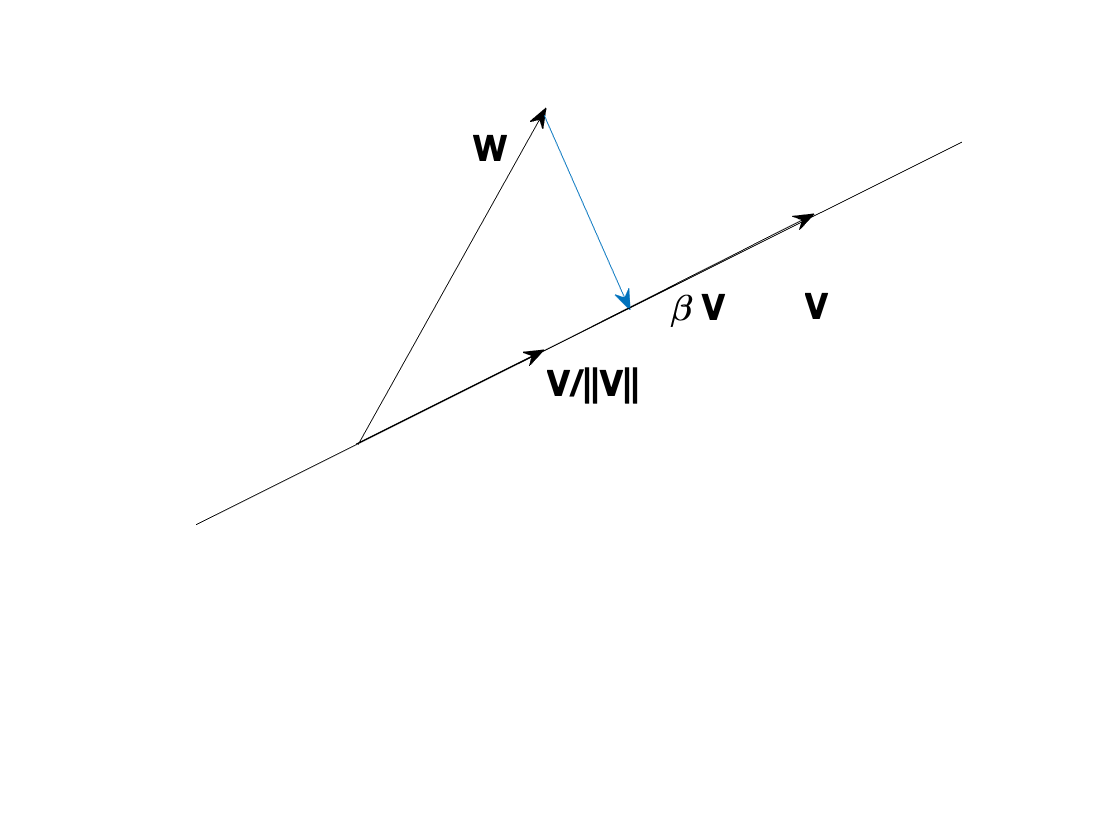
\includegraphics[scale=0.15]{proywsobrev.png}
\caption{Proyección de $\wb$ sobre la recta generada por $\vb$.}
 \label{fig:proyusobrev}
\end{figure}

\tcc
De los argumentos previos vemos que \emph{en una base ortonormal}, las proyecciones ortogonales de un vector $\wb$ sobre los elementos de la base nos dan sus coordenadas en esa base. Eso  es justamente a lo que estamos acostumbrados en la base can\'onica.
\etcc
Otro hecho de gran importancia es la generalización del teorema de Pitágoras en cualquier dimensión si tenemos una base ortonormal. Esto es, de la expresión \eqref{eq:escritura_ort}, tenemos que el cuadrado de la longitud de $\wb$ (el cuadrado de la ``hipotenusa'') es, por un lado
$$\|\wb\|^2_2=\wb^*\wb$$ y por el otro
$$
(\sum_{i=1}^n\alpha_i\vb_i)^*(\sum_{i=1}^n\alpha_i\vb_i)=(\sum_{i=1}^n\overline{\alpha_i}\vb_i^*)(\sum_{i=1}^n\alpha_i\vb_i)=
\sum_{i,j=1}^n\overline{\alpha_j}\alpha_i\vb_j^*\vb_i=\sum_{i=1}^n\overline{\alpha_i}\alpha_i=\sum_{i=1}^n|\alpha_i|^2,
$$
es decir el cuadrado de la suma de las longitudes de las coordenadas (los ``catetos'').
Para resaltar este hecho que usaremos en lo sucesivo, lo recuadramos,
\tcc
\begin{rem}
\label{obs:pitagoras}
En toda base ortonormal $\mathcal{B}=\{\vb_1,\cdots,\vb_n\}$, si
$$
\wb=\sum_{i=1}^n\alpha_i\vb_i,
$$
entonces
$$
\|\wb\|^2=\sum_{i=1}^n|\alpha_i|^2.
$$
\end{rem}
\etcc
Mas adelante volveremos sobre el tema de las proyecciones.

Para finalizar la sección de producto interno definimos

\tccdefi \begin{defi}
 Una matriz $\Ab\in \Cnn$ se dice \emph{Hermitiana} si $\Ab=\Ab^*$. En el caso de que $\Ab\in \Rnn$, $\Ab$ se dice \emph{simétrica}.
\end{defi}
\etcc
Si $\Ab\in \Knn$ es Hermitiana, entonces, para todo $\vb\in \Kn$, $\vb^*\Ab\vb\in \R$. En efecto, por un lado, debido a las dimensiones de los elementos que aparecen en el producto, se tiene  $z=\vb^*\Ab\vb\in \K$, por otro lado puesto que
$$\overline{\vb^*\Ab\vb}=(\vb^*\Ab\vb)^*=\vb^*\Ab^*(\vb^*)^*=\vb^*\Ab\vb,$$
resulta de la primera y ultima expresión de la cadena de igualdades que $\overline{z}=z$, es decir $z\in \R$.

\tccdefi
\begin{defi}
\label{def:positiva}
 Una matriz $\Ab\in \Cnn$ ($\Ab\in \Rnn$)  se dice \emph{definida positiva} si es Hermitiana (simétrica) y además $\vb^*\Ab\vb>0$ para todo $\vb\neq 0$.  Si por otro lado $\vb^*\Ab\vb\ge0$ para todo $\vb$, la matriz se dice \emph{semi definida} positiva.
\end{defi}
\end{tcolorbox}


\section{Normas de matrices}
Dada una matriz $A \in \K^{n \times m}$, se la puede pensar pensar como un vector de $\K^{nm}$ y en consecuencia se aplicaría a las matrices todo lo que hemos desarrollado para normas vectoriales.  Sin embargo, salvo casos excepcionales\footnote{Como la norma de Frobenius que veremos mas adelante.}, esta normas no son de gran utilidad en el contexto de las matrices. Esto es debido a que nos interesa estudiarlas desde la perspectiva  de las trasformaciones lineales asociadas. Por esta razón se introducen las normas subordinadas.

Dada una matriz $\Ab \in \K^{n \times m}$, y un par de normas vectoriales $\|\cdot\|_n,\|\cdot\|_m$ en $\K^n$ y $\K^m$ respectivamente, definimos
$$
\|\Ab\|_{n,m} = \max_{\cero \neq \xb \in \K^m} \frac{\|\Ab\xb\|_n}{\|\xb\|_m} = \max_{\xb \in \K^m, \|\xb\|_m = 1} \|\Ab\xb\|_n.
$$
Un caso usual en este curso es que la matriz sea cuadrada $\Ab \in \K^{n \times m}$ y en ese caso usamos una sola norma vectorial $\|\cdot\|$
\tccdefi
\begin{equation}
 \label{eq:defidenormaA}
\|\Ab\| = \max_{\cero \neq \xb \in \K^m} \frac{\|\Ab\xb\|}{\|\xb\|} = \max_{\xb \in \K^m, \|\xb\| = 1} \|\Ab\xb\|.
\end{equation}
\etcc

Estas normas matriciales se dicen \emph{subordinadas} a la norma vectorial $\|\cdot\|$ que estamos utilizando
en el espacio $\Kn$ . De su definición vemos que  la norma (subordinada) de una matriz mide en qué proporción puede aumentar como máximo la norma de un vector $\xb$ al multiplicarlo por $\Ab$.

\begin{ej}
Sea $\Ab\in \Knn$ y $\|\cdot\|$ una norma en $\Kn$, entonces
 \eqref{eq:defidenormaA} define una norma.
\end{ej}
\begin{ej}
\label{ej:idnorma1}
Sea $\Ib\in \Knn$ la identidad, entonces
 $\|\Ib\|=1$ para toda norma subordinada (siempre que pensemos $\Kn$ con la misma norma vectorial como espacio de partida y llegada de la transformación $\Ib:\Kn\to \Kn$).
\end{ej}

También resulta inmediato de la definición que para todo $\xb$
\begin{equation}
 \label{eq:acotacionoperador}
\|\Ab\xb\|\le \|\Ab\|\|\xb\|.
\end{equation}
De aquí se obtiene la siguiente propiedad. Para todo par de matrices\footnote{Como se desprende de la cuenta,  también vale para matrices rectangulares, siempre que pueda hacerse el producto $\Ab\Bb$.} $\Ab, \Bb\in \Knn$, y toda \emph{norma subordinada}
\begin{equation}
 \label{eq:prodnormas}
\|\Ab\Bb\|\le \|\Ab\|\|\Bb\|.
\end{equation}
En efecto,
dos aplicaciones sucesivas de \eqref{eq:acotacionoperador} da
$$
 \|\Ab\Bb\|=\max_{\|\xb\|=1}
\|\Ab\Bb\xb\|\le \max_{\|\xb\|=1}
\|\Ab\|\|\Bb\xb\|\le \max_{\|\xb\|=1}\|\Ab\|\|\Bb\|\|\xb\|=\|\Ab\|\|\Bb\|,$$
que prueba \eqref{eq:prodnormas}.
Aplicando sucesivamente \eqref{eq:prodnormas}, vemos que para toda matriz cuadrada y para todo $k\in\N$, vale\footnote{Que ocurre si $k\in \mathbb{Z}$ con $k<0$?. Por ejemplo, cuando $\Ab$ es invertible sabemos darle sentido a $\Ab^{-1}$ como la inversa de $\Ab$.
Por lo tanto $\Ib=\Ab\Ab^{-1}$ de donde $1\le \|\Ab\|\|\Ab^{-1}\|$  (hemos usado aquí el Ejercicio \ref{ej:idnorma1}) y de ahí $\|\Ab\|^{-1}\le \|\Ab^{-1}\|$. Es decir al revés que en  \eqref{eq:normasypotencias}.  Piense que ocurre en general. Defina primero $\Ab^{k}$ con $k<0$. Como ayuda pregúntese que será por ejemplo $\Ab^{-3}$?. Vea que puede pensarlo como $\Ab^{-3}:=\left(\Ab^{-1}\right)^3$, es decir $\Ab^{-3}=\Ab^{-1}\Ab^{-1}\Ab^{-1}$. Pero otro lado $\Ab^3\left(\Ab^{-1}\Ab^{-1}\Ab^{-1}\right)=\Ib$, lo que dice que la primera definición coincide con $(\Ab^3)^{-1}$. Use estas consideraciones para responder la pregunta.}
\begin{equation}
 \label{eq:normasypotencias}
\|\Ab^k\|\le \|\Ab\|^k.
 \end{equation}
En algunos pocos casos es posible calcular explícitamente la expresión de $\|\Ab\|$.

\begin{ejemplo}
Consideremos en $\K^n$ la norma $\|\cdot\|_\infty$. Para $\Ab\in \Knn$ se tiene\footnote{También vale la demostración en el caso de matrices rectangulares.}
\tcc
$$
 \|\Ab\|_\infty=\max_{1\le i\le n}\{\sum_{j=1}^{n} |a_{ij}|\}.
$$
\etcc
\begin{proof}
 Lo vemos para $\K=\R$. Debemos calcular
$$\|\Ab\|_\infty =
\max_{\xb \in \R^n, \|\xb\|_\infty = 1} \|\Ab\xb\|_\infty.
 $$
 Llamemos $k$ a la fila donde ser realiza el máximo, es decir
 $$
 \max_{1\le i\le n}\{\sum_{j=1}^{n} |a_{ij}|\}=\sum_{j=1}^{n} |a_{kj}|,
 $$
 (si hay más de una tomamos cualquiera). Podemos suponer que
 $\sum_{j=1}^{n} |a_{kj}|>0$ de otro modo el resultado es inmediato. Llamemos $\zb$ al vector de los signos de los elementos de esa fila $\zb=(sg(a_{k,1}),\cdots ,sg(a_{k,n})$. Si algún $a_{k,i}=0$ tomamos $sg(a_{k,1})=0$. Como la fila no es nula, $\zb\neq\cero$. Luego $\|\zb\|_\infty=\max_{1\le i\le n}\{|z_i|\}=1$, y  haciendo
 $$
\|\Ab\|_\infty =\max_{\xb \in \R^n, \|\xb\|_\infty = 1} \|\Ab\xb\|_\infty
 \ge \|\Ab\zb\|_\infty\ge \sum_{j=1}^n a_{i,j}sg(a_{i,j})=\sum_{j=1}^n |a_{i,j}|=\max_{1\le i\le n}\{\sum_{j=1}^{n} |a_{ij}|\},
 $$
 lo que prueba una desigualdad. Para a otra desigualdad, sea $\xb\in \R^n$ tal que $\|\xb\|_\infty=1$, luego para todo $1\le j\le n$ $|x_j|\le \|\xb\|_\infty=1$ y entonces, para cualquier elemento $i$ del vector $\Ab\xb$
$$
|[\Ab\xb]_i|=|\sum_{j=1}^na_{i,j}x_j |\le \sum_{j=1}^n|a_{i,j}|\le \max_{1\le i\le n}\{\sum_{j=1}^{n} |a_{ij}|\},
$$
lo que da la otra desigualdad y demuestra el caso $\K=\R$.
El caso $\K=\C$ sale del mismo modo recordando que si $z\in \C$ y $z=|z|e^{i\theta}$, se tiene que $ze^{-i\theta}=|z|$ y $|e^{i\theta}|=1$.
\end{proof}
Análogamente para la norma$-1$ se tiene
\end{ejemplo}

\begin{ejemplo}
Consideremos en $\K^n$ la norma $\|\cdot\|_1$. Para $\Ab\in \Knn$ se tiene\footnote{También vale  en el caso de matrices rectangulares.}
\tcc
$$
 \|\Ab\|_1=\max_{1\le j\le n}\{\sum_{i=1}^{n} |a_{ij}|\}.
$$
\etcc
\end{ejemplo}
Un caso de mucha importancia para nosotros es la norma matricial subordinada a la norma$-2$.
Comencemos calculando un caso elemental: la norma$-2$ de una matriz unitaria/ortogonal (Definición \ref{def:de_unitaria}).
Supongamos que $\Qb\in \Knn$ y $\Qb^*\Qb=\Ib$, luego, para todo$\xb\in\Kn$
$$
\|\Qb\xb\|_2^2=(\Qb\xb)^*\Qb\xb=\xb^*\xb=\|\xb\|^2_2,
$$
es decir que
\begin{equation}
\label{eq:isometria}
\|\Qb\xb\|_2=\|\xb\|_2, \, \forall \xb\in \K^n.
\end{equation}
 Vemos que las matrices unitarias son \emph{isometrías}, es decir, no cambian las longitudes. Tampoco cambian los ángulos ya que preservan el producto interno, propiedad que resaltamos a continuación 
 \tcc
 \begin{equation}
 \label{eq:preservaPI}
\langle \Qb\vb,\Qb\wb \rangle=(\Qb\vb)^*\Qb\wb=\vb^*\wb=\langle \vb,\wb \rangle.
 \end{equation}
\etcc
Estas propiedades definen a los \emph{movimientos rígidos}. De \eqref{eq:isometria}, tenemos
$$
\|\Qb\|_2=\sup_{\xb\neq\cero}\frac{\|\Qb\xb\|_2}{\|\xb\|_2}=1,
$$
lo que les da su nombre a las matrices unitarias.
\begin{ej}Verificar que la matriz
$$
\Ab = \begin{pmatrix}
1 & 0 & 0 \\ 0 & \cos \alpha & -\sin \alpha \\ 0 & \sin \alpha & \cos \alpha
\end{pmatrix}
$$
es una matriz ortogonal para cualquier valor de $\alpha$. Interpretar geométricamente la transformación lineal $\Ab\xb$.
\end{ej}

Como ya hemos señalado, las normas subordinadas son las mas útiles. Sin embargo la norma euclídea aplicada a matrices -que es no subordinada- tiene importantes aplicaciones y un nombre propio.
\tccdefi
\begin{defi}
 Dada $\Ab\in \K^{n\times m}$ definimos la norma de Frobenius
 $$
 \|\Ab\|_F=\sqrt{\sum_{1\le i\le n}\sum_{i\le j\le m} |a_{i,j}|^2}
 $$
\end{defi}
\etcc
Notar que
$$
\|\Ab\|_F=\sqrt{tr(\Ab^T\Ab)},
$$
donde $tr$ indica el operador traza (la suma de los elementos de la diagonal). Las normas no subordinadas de matrices no suelen cumplir con la desigualdad \eqref{eq:prodnormas}. La norma de Frobenius es una excepción, gracias a la desigualdad de Cauchy-Schwarz. En efecto, dados\footnote{El siguiente argumento vale también para matrices rectangulares.}
$\Ab,\Bb\in \Knn$, consideremos el elemento $i,j$ de la  matriz producto
$$
|[\Ab\Bb]_{i,j}|^2\le |(\sum_{l=1}^n\Ab_{i,l}\Bb_{l,j})|^2\le (\sum_{1=1}^n\Ab_{i,l}^2)(\sum_{1=1}^n\Bb_{l,j}^2),
$$
donde hemos usado la Proposición \ref{prop:CS} en la última desigualdad. Sumando en $i$ y en $j$ se tiene el resultado deseado
$$
\|\Ab\Bb\|_F^2=\sum_{1\le i,j\le n}|[\Ab\Bb]_{i,j}|^2\le\sum_{1\le i\le n}\sum_{1\le j\le n}(\sum_{1=1}^n\Ab_{i,l}^2)(\sum_{1=1}^n\Bb_{l,j}^2)=
\|\Ab\|_F^2\|\Bb\|_F^2,
$$
esto es
\tcc
$$\|\Ab\Bb\|_F\le \|\Ab\|_F\|\Bb\|_F.$$
\etcc
Cerramos esta sección con propiedades de las normas de matrices unitarias (algunas las hemos ya probado pero las ponemos en recuadro para recordarlas).
De todas la matrices, las unitarias poseen propiedades especiales que las hacen muy favorables para su uso en los algoritmos.
\tcc
\begin{prop}
 \label{prop:unitarias}
 Sea $\Ab\in \K^{n\times m}$, $\Qb\in \Knn$, $\Qb$ unitaria/ortogonal, resulta
 \begin{enumerate}
  \item $\forall \vb\in \Kn$
  $\|\Qb\vb\|_{2}=\|\vb\|_2$
  \item $\|\Qb\|_{2}=1$
  \item $\|\Qb\Ab\|_2=\|\Ab\|_2$
  \item $\|\Qb\Ab\|_F=\|\Ab\|_F$
 \end{enumerate}
\end{prop}
\etcc
\begin{proof} Las propiedades $(1)$ y $(2)$ ya las hemos probado.

Para $(3)$, notemos que por $(1)$ se tiene
 $$\|\Qb\Ab \|_{2}=sup_{\vb, \|\vb\|_2=1}
 \|\Qb\Ab \vb\|_{2}=sup_{\vb, \|\vb\|=1}\|\Ab\vb\|_2=\|\Ab\|_2.
 $$
 Finalmente, para $(4)$ escribimos
 $$
 \|\Qb\Ab\|_F^2=tr((\Qb\Ab)^*(\Qb\Ab))=tr(\Ab^*\Ab)=\|\Ab\|_F^2.
 $$\end{proof}


\section{Condicion de Matrices}
Sea $\Ab\in \R^{n\times m}$,  queremos estudiar en más detalle la condición de evaluar $\Ab\vb$ (pensado como transformación lineal). Notemos que podemos hacerlo con bastante en general aprovechando la linealidad.
En efecto, para una perturbación arbitraria $\hb$ de $\vb$ tenemos que el error relativo de evaluar en $\vb$ (asumiendo que $\vb\notin Nu(\Ab)$) puede escribirse
$$
\frac{\|\Ab(\vb+\hb)-\Ab\vb \|}{\|\Ab\vb\|}=\frac{\|\Ab\hb\|}{\|\Ab\vb\|},
$$
y este valor, respecto del error relativo en $\vb$ resulta
$$
\frac{\frac{\|\Ab\hb\|}{\|\Ab\vb\|}}{\frac{\|\vb\|}{\|\hb\|}}=\frac{\|\Ab\hb\|}{\|\hb\|}\frac{\|\vb\|}{\|\Ab\vb\|}\le \|\Ab\|\frac{\|\vb\|}{\|\Ab\vb\|}.
$$
El número que está a la derecha es independiente de $\hb$ y podemos usarlo como representante de la condición de evaluar $\Ab$ en $\vb$ y de hecho vemos que  coincide con la expresión sugerida para la condición en el caso general  (i.e. $
\frac{\|x_0\|\|Df(x_0)\|}{\|f(x_0)\|}
$). Si quisieramos una expresión independiente de $\vb$ que podríamos hacer?. En el caso en que $n=m$ y $\Ab$ sea invertible, podemos llamar $\wb=\Ab\vb$ y el cociente $\frac{\|\vb\|}{\|\Ab\vb\|}$ puede acotarse idependiente de $\vb$
$$
\frac{\|\vb\|}{\|\Ab\vb\|}=
\frac{\|\Ab^{-1}\wb\|}{\|\wb\|}
\le \|\Ab^{-1}\|.$$
En definitiva hallamos un número que mayora a la condición de evaluar en $\vb$ para todo $\vb$ y este es
$$
\|\Ab\|\frac{\|\vb\|}{\|\Ab\vb\|}\le \|\Ab\|\|\Ab^{-1}\|.
$$
Notemos que argumentando con $\Ab^{-1}$, vemos que el mismo número mayora a la condición de evaluar $\Ab^{-1}\wb$. Esto motiva la siguiente definición.

\begin{defi}{(Condición de una matriz)}
Dada $\Ab\in \Knn$ invertible definimos la condición de $\Ab$, $\kappa(\Ab)$, asociada a una norma subordinada $\|\cdot\|$, como
$$
\kappa(\Ab)=\|\Ab\|\|\Ab^{-1}\|.
$$
Si $\Ab$ no es invertible definimos $\kappa(\Ab)=+\infty$.

\end{defi}
Que ocurre si $\Ab\in \K^{n\times m}$? podremos definir algo similar?.  Volveremos sobre este caso mas adelante cuando definamos la \emph{pseudoinversa}.
\begin{remark}
\label{rem:deCondicion}
Observemos que
\begin{enumerate}
 \item La condición de una matriz depende de la norma matricial elegida. Sin embargo, como en dimensión finita todas las normas son equivalentes las condiciones son equivalentes.
\item Para todo $\cero\neq \alpha\in \K$, $\kappa(\alpha\Ab)=\kappa(\Ab)$.
\item $\kappa(\Ib)=1$ para toda norma.
 \item Como consecuencia del ítem previo, para toda norma, $1\le \kappa(\Ab)$.
\item Para toda $\Qb$ unitaria/ortogonal
$\kappa(\Qb)=1$. (ver item (2) en Proposición \ref{prop:unitarias})
\item $\kappa(\Ab)=\kappa(\Ab^{-1})$
\end{enumerate}
\end{remark}
Consideremos por un segundo los problemas que pueden aparecer cuando resolvemos un sistema
$$
\Ab\xb=\bb
$$
con $\bb\neq\cero$ y $\Ab$ invertible.
Por un lado tenemos que considerar que tanto $\Ab$ como $\bb$ se almacenaran con errores. En general entonces estaremos resolviendo otro problema
$$
(\Ab+\Delta\Ab)(\xb+\Delta \xb)=
\bb +\Delta \bb.
$$
Asumiendo que procedemos a resolver el problema con aritmética exacta (no hay otras fuentes de error) nos interesa ver el impacto en el error $\Delta \xb$ debido a los errores $\Delta \Ab,\Delta \bb$.

Tenemos, usando que $\Ab\xb=\bb$
$$
\Delta \Ab\xb+\Ab\Delta\xb+\Delta \Ab\Delta \xb=\Delta \bb.
$$
Procediendo \emph{informalmente}, despreciamos el término de ``segundo orden'' $\Delta \Ab\Delta \xb$ y resulta
$$
\Delta \Ab\xb+\Ab\Delta\xb \sim \Delta \bb.
$$
de donde
$$
\Delta \xb\sim \Ab^{-1}\Delta \bb-\Ab^{-1}\Delta \Ab\xb,
$$
y usando que $\|\Ab\|\neq 0$,
$$
\|\Delta \xb\|\lesssim \|\Ab^{-1}\|\|\Delta \bb\|+\|\Ab^{-1}\|\Delta \Ab\|\|\xb\|=\|\Ab^{-1}\|\frac{\|\Delta \bb\|}{\|\bb\|}\|\bb\|+\|\Ab^{-1}\|\frac{\|\Delta \Ab\|}{\|\Ab\|}\|\Ab\|\|\xb\|,
$$
usando que $\|\bb\|\le \|\Ab\|\|\xb\|$ y diviendo por $\|\xb\|\neq \cero$ tenemos
$$\frac{\|\Delta \xb\|}{\|\xb\|}\lesssim \kappa(\Ab)\left(\frac{\|\Delta \bb\|}{\|\bb\|}+ \frac{\|\Delta \Ab\|}{\|\Ab\|}\right).$$
Lo que dice que el error  relativo generado en la solución  se acota en terminos de los errores relativos en los datos por la condición de la matriz.

Observar que en caso de ser $\Delta \Ab=\cero$ (no hay error en la matriz) podemos reemplazar $\lesssim$ con $\le$ y queda
$$\frac{\|\Delta \xb\|}{\|\xb\|}\le \kappa(\Ab)\frac{\|\Delta \bb\|}{\|\bb\|}.$$
De hecho, escribiendo
$\Ab^{-1}\bb=\xb,$ y $\Ab^{-1}(\bb+\Delta\bb)=\xb+\Delta \xb$ se puede argumentar con $\Ab^{-1}$ y por (6) de la Observación \ref{rem:deCondicion}, se ve que
$$\frac{\|\Delta \bb\|}{\|\bb\|}\le \kappa(\Ab)\frac{\|\Delta \xb\|}{\|\xb\|}.$$
Resumiendo
\tcc
$$\frac{1}{\kappa(\Ab)}\frac{\|\Delta \bb\|}{\|\bb\|}\le \frac{\|\Delta \xb\|}{\|\xb\|}\le \kappa(\Ab)\frac{\|\Delta \bb\|}{\|\bb\|}.$$
\etcc
\begin{ej}
 Verifique con ejemplos que las desigualdades previas se alcanzan (Sug.: use matrices diagonales adecuadas).
\end{ej}
Teniendo en cuenta el ejercicio previo, vemos que la cota superior puede alcanzarse en la pŕactica. En particular nos dice de un modo simplificado que podemos perder $log_{10}(\kappa(\Ab))$ dígitos significativos al resolver el sistema\footnote{Por ejemplo, si $\kappa(\Ab)\sim 10^{16}$ no tenemos la garantía de tener ni un dígito correcto en nuestro resultado.}.

El siguiente resultado da una idea cualitativa de $\kappa(\Ab)$ como el recíproco de la distancia relativa de $\Ab$ a las matrices singulares.
\begin{teo}
 $\Ab\in \Rnn$, se tiene,
 \begin{equation}
 \label{eq:minimoasing}
\frac{1}{\kappa(\Ab)}=\inf_{\Bb\,  \mbox{singular}} \frac{\|\Ab-\Bb\|}{\|\Ab\|},
 \end{equation}
 y en donde asumimos $\frac{1}{\kappa(\Ab)}=0$ en caso de que $\Ab$ no sea invertible.
 \end{teo}
 \begin{proof}
  Si $\Ab$ es no invertible el resultado es evidente. Supongamos entonces que $\Ab$ es invertible. Probaremos únicamente que vale  el $\le$  en \eqref{eq:minimoasing}.

  Sea $B\in \Rnn$ una matriz singular cualquiera. Tomemos $\cero\neq \vb\in Ker(\Bb)$, y definamos $\cero\neq\wb=\Ab\vb$. Se tiene
  $$
  0\neq \|\wb\|=\|(\Ab - \Bb)\vb\|\le \|\Ab-\Bb\|\|\Ab^{-1}\wb\|\le \|\Ab-\Bb\|\|\Ab^{-1}\|\|\wb\|,
  $$
  dividiendo por $\|\Ab\|\|\Ab^{-1}\|\|\wb\|\neq 0$ se obtiene
  $$
\frac{1}{\kappa(\Ab)}\le  \frac{\|\Ab-\Bb\|}{\|\Ab\|},
 $$
 y por ser $\Bb$ arbitrario
 $$
\frac{1}{\kappa(\Ab)}\le \inf_{\Bb\,  \mbox{singular}} \frac{\|\Ab-\Bb\|}{\|\Ab\|},
 $$
 \end{proof}
El resultado anterior dice que un número condición grande significa cercanía -relativa- a las matrices singulares. Es importante remarcar que el determinante  no es la herramienta adecuada para medir esa cercanía, pues el ítem (2) de la Observación \ref{rem:deCondicion} dice que el número de condición no cambia por múltiplos de una matriz sin embargo $\det(\alpha\Ab)=\alpha^n\det(\Ab)$ que tiende a cero si $\alpha\to 0$.
\section{Proyecciones y Proyectores}
\label{sec:proyectores}
Observemos otra forma equivalente de escribir la proyección ortogonal de $\wb$ sobre el subespacio generado por $\vb$ (ver \eqref{eq:proy_forma1}):
\begin{equation}
 \label{eq:proy_forma2}
 \Pb_{\vb}(\wb)=\frac{\vb}{\|\vb\|_2}\frac{\vb^*}{\|\vb\|_2}\wb,
\end{equation}
que puede verse como una aplicación lineal de matriz  $\frac{\vb\vb^*}{\|\vb\|_2\|\vb\|_2}$.
\tcc
Notar que la matriz $\frac{\vb\vb^*}{\|\vb\|_2\|\vb\|_2}$ , asociada a la proyección $\Pb_{\vb}$, tiene rango $1$, de hecho las columnas son todas múltiplos de $\vb$.
\etcc

Un caso notable es cuando $\vb$ es de norma uno. En ese caso
\begin{equation}
 \label{eq:proy_forma2_norma1}
 \Pb_{\vb}(\wb)=\vb\vb^*\wb,
\end{equation}
teniendo esto en mente volvamos un segundo a la ecuación \eqref{eq:escritura_ort}. Si en vez de una base completa solo contamos con un conjunto de vectores ortonormales $\mathcal{C}=\{\vb_1,\cdots,\vb_k\}\subset \Kn$, $k<n$, y llamamos $\mathcal{S}=\langle \vb_1,\cdots,\vb_k\rangle$ al subespacio generado por esos vectores, vemos  que la expresión
\begin{equation}
 \label{eq:proysobreS}
\Pb_{\mathcal{S}}(\wb)=\sum_{1\le i\le k}\Pb_{\vb_i}(\wb).
\end{equation}
verifica
$$
(\wb-\Pb_{\mathcal{S}}(\wb))\perp \vb_j, \qquad \forall 1\le j\le k,
$$
pues
$$
\vb_j^*(\wb-\Pb_{\mathcal{S}}(\wb))=\vb_j^*\wb -\sum_{1\le i\le k}\vb_j^*\Pb_{\vb_i}(\wb)= \vb_j^*\wb-\vb_j^*\wb=0.
$$
Luego, por ser ortogonal a todos los generadores de $\mathcal{S}$ lo será a todos lo elementos de $\mathcal{S}$. En otras palabras, teniendo una base ortonormal de $\mathcal{S}$ es muy fácil construir la proyección ortogonal de un elemento $\wb$ sobre  $\mathcal{S}$ usando la expresión \eqref{eq:proysobreS}.
Como además cada $\Pb_{\vb_i}$ admite una representación matricial, lo mismo ocurre con  $\Pb_{\mathcal{S}}$,
$$\Pb_{\mathcal{S}}=
\begin{pmatrix}
&|&&|&&|&\\
&|&&|&&|&\\
\vb_1&|&\vb_2&|&\cdots&|&\vb_k\\
&|&&|&&|&\\
&|&&|&&|&\\
\end{pmatrix}
\begin{pmatrix}
&&&\vb_1^*&&&\\
-&-&-&-&-&-&-\\
&&&\vb_2^*&&&\\
-&-&-&-&-&-&-\\
 &&&\vdots&&& \\
-&-&-&-&-&-&-\\
&&&\vb_k^*&&&
\end{pmatrix}.
$$
En efecto, tomando $w\in \K^n$ tenemos, llamando $\Mb$ a la matriz anterior que
$$
\Mb\wb=\begin{pmatrix}
&|&&|&&|&\\
&|&&|&&|&\\
\vb_1&|&\vb_2&|&\cdots&|&\vb_k\\
&|&&|&&|&\\
&|&&|&&|&\\
\end{pmatrix}
\begin{pmatrix}
 \vb_1^*\wb\\
 \vb_2^*\wb\\
 \vdots \\
 \vb_k^*\wb\\
 \end{pmatrix}
=\sum_{1\le i\le k}\vb_i\vb_i^*\wb
=\sum_{1\le i\le k}\Pb_{\vb_i}(\wb).
$$
es decir que coincide con \eqref{eq:proysobreS}.
\begin{figure}
\includegraphics[scale=0.25]{proyS.png}
%\end{center}
 \label{fig:proyecsobreS}
 \caption{Proyección ortogonal de $\wb$ sobre el subespacio $\mathcal{S}$.}
%\begin{center}
\end{figure}

Por lo tanto, si queremos obtener la proyección ortogonal de un vector sobre un subespacio $\mathcal{S}$ podemos hacerlo a través de una base ortonormal de $\mathcal{S}$. Sabemos que obtener una familia de generadores de $\mathcal{S}$, $l.i.$ es relativamente sencillo. Sería ideal tener un método para obtener, a partir de esa familia, un sistema de generadores ortonormales. Veamos como hacerlo.

Dada una familia de vectores $\{\vb_1, \vb_2, ...,\vb_n\}$ linealmente independientes. La ortonormalización de Gram-Schmidt
es un algoritmo que produce una sucesión de vectores ortonormales  $\{\qb_1,\qb_2,...,\qb_n\}$ del siguiente modo
El proceso consiste en restarle a cada vector $\vb_i$ sus componentes en los vectores anteriores.

Podemos construir primero una familia ortogonal y luego normalizarla (o normalizarla durante la construcción). Llamemos $\ub_i$ a los ortogonalizados, el método es el siguiente
\begin{itemize}
\item   $\ub_1 = \vb_1$, $\ub_1 = \frac{\ub_1}{\|\ub_1\|}$
\item   $\ub_2 = \vb_2 -\Pb_{\ub_1}(\vb_2)$
$\ub_2 = \frac{\ub_2}{\|\ub_2\|}$
\item   $\ub_3 = \vb_3 -
\Pb_{\ub_1}(\vb_3)-\Pb_{\ub_2}(\vb_3)$, $\ub_3 = \frac{\ub_3}{\|\ub_3\|}$
\item   $\dots$
\item $\ub_k = \vb_k - \sum_{i = 1}^{k-1} \Pb_{\ub_i}(\vb_k)$, $\ub_k = \frac{\ub_k}{\|\ub_k\|}$.
\end{itemize}
Notemos que el algoritmo solo puede detenerse (es decir alcanzar una operación inválida) si y solo si algún $u_j=\cero$ para algún $j$. Pero si esto ocurre, significa que $\vb_j$ es combinación lineal de $\{\vb_1,\vb_2\cdots,\vb_{j-1}\}$\footnote{En efecto, observar que mientras no se detenga el algoritmo $\langle\ub_1,\ub_2,...,\ub_{j}\rangle=\langle\vb_1,\vb_2,..., \vb_{j}\rangle$ para todo $1\le j$.} lo cual contradice el presupuesto de ser $\{\vb_1, \vb_2, ...,\vb_n\}$ linealmente independientes.

Escribimos debajo el algoritmo de forma compacta llamando $\qb_i$ a los vectores ortonormales obtenidos\footnote{Notación compatible con $\Qb$ para las matrices otrogonales/unitarias.}.


\begin{center}
\begin{tcolorbox}[width=\linewidth/3]
\begin{center}
{\bf Gramm-Schmidt}
\end{center}


{\bf for} j=1 {\bf to} n

\qquad $\vb_j=\ab_j$

\qquad {\bf for} i=1 to j-1

\qquad\qquad $r_{i,j}=\qb_i^*\ab_j$

\qquad\qquad  $\vb_j=\vb_j-r_{i.j}
\qb_i$


\qquad$r_{j,j}=\|\vb_j\|_2$

\qquad$\qb_{j}=\vb_j/r_{j,j}$

\end{tcolorbox}
\end{center}
Esta familia de vectores verifica,
\begin{itemize}
 \item $\{\qb_1,\qb_2,...,\qb_k\}$ es ortonormal.
 \item $\langle\qb_1,\qb_2,...,\qb_k\rangle=\langle\vb_1,\vb_2,..., \vb_k\rangle$ para todo $1\le k\le n$.
\end{itemize}

Ya hemos hemos notado que las proyecciones ortogonales de vectores sobre subespacios  resultaban aplicaciones lineales.  Vamos a describir las matrices asociadas a esas aplicaciones.
\tccdefi
\begin{defi}
Una matriz $\cero \neq \Pb\in \Knn$ se dice un proyector si
$\Pb^2=\Pb$.
\end{defi}
\etcc

Notar que  dados dos subespacios $S_1,S_2$ tales que $S_1\oplus S_2=\Kn$, siempre es posible construir un proyector $\Pb$ tal que $Im(\Pb)=S_1$ y $Nu(\Pb)=S_2$. En efecto, como los subespacios están en suma directa, para todo $\vb\in \Cn$ existen únicos $\vb_i\in S_i$ tales que
$\vb=\vb_1+\vb_2$. Definiendo $\Pb\vb=\vb_1$ obtenemos el proyector buscado.

Si $\Pb$ es un projector y $\Pb\neq \Ib$ entonces $\Ib-\Pb$ también es un proyector denominado \emph{proyector complementario}.

Un proyector $\Pb$ deja invariante su rango, ya que si $\vb\in Rg(\Pb)$ entonces $\exists \wb$ tal que  $\Pb\wb=\vb$, por lo que
$$
\Pb\vb=\Pb\Pb\wb=\Pb\wb=\vb,
$$
decimos que $\Pb$ proyecta sobre su rango $Rg(\Pb)$.

Notemos que
$$Rg(\Ib-\Pb)=Ker(\Pb),$$
ya que si $\wb\in Rg(\Ib-\Pb)$, es $\wb=\vb-\Pb\vb$ de donde $\Pb\wb=\cero$, i.e. $\wb\in Ker(\Pb)$. Por otro lado, si $\wb\in Ker(\Pb)$,
$Rg(\Ib-\Pb)\ni (\Ib-\Pb)\wb=\wb$. El argumento anterior también implica
$$Rg(\Pb)=Ker(\Ib-\Pb).$$
Por otro lado, se observa trivalmente que  $Ker(\Ib-\Pb)\cap Ker(\Pb)=\{\cero\}$ y entonces
$$Rg(\Pb)\cap Ker(\Pb)=\{\cero\}.$$
Esto dice que
$$
\Kn=Ker(\Pb)\oplus Rg(\Pb).
$$
\tccdefi
\begin{defi}
 Un proyector $\Pb$ se dice \emph{ortogonal} si $Ker(\Pb)\perp Rg(\Pb)$. En otro caso, se dice \emph{oblícuo}.
\end{defi}
\etcc
\tcc
\begin{prop}
\label{prop:ortssiautoadjunto}
Un proyector $\Pb$ es ortogonal sí y solo sí $\Pb=\Pb^*$.
\end{prop}
\etcc
\begin{proof}
 Si $\Pb$ es ortogonal, $\forall, \vb,\wb$
 $$
 0=((\Ib-\Pb)\vb)^*\Pb\wb=\vb^*(\Ib-\Pb)^*\Pb\wb,
 $$
 lo que indica que
 $$
 \cero=(\Ib-\Pb)^*\Pb=\Pb-\Pb^*\Pb,
 $$
 es decir $\Pb=\Pb^*\Pb$ y en particular resulta $\Pb=\Pb^*$.

 Recíprocamente, si $\Pb=\Pb^*$,
 $$
 ((\Ib-\Pb)\vb)^*\Pb\wb=\vb^*(\Ib-\Pb)^*\Pb\wb=\vb^*(\Pb-\Pb^2)\wb=0,
 $$
 $\forall, \vb,\wb$, lo que dice que $\Pb$ es ortogonal.
\end{proof}

\tcc
\begin{teo}
 Sea $\Pb$ un proyector. Son equivalentes:
 \begin{enumerate}
  \item $\Pb$ es ortogonal
  \item $\|\vb\|_2=\|(\Ib-\Pb)\vb\|_2+\|\Pb\vb\|_2$ para todo $\vb$
  \item $\|\Pb\|_2=1$
 \end{enumerate}
\end{teo}
\etcc
\begin{proof}
 $(1)\rightarrow (2)$: para todo $\vb$ escribimos
 $$
 \vb=(\Ib-\Pb)\vb+\Pb\vb,
 $$
 y como por ser proyector $Im(\Ib-\Pb)=Nu(\Pb)\perp Im(\Pb)$, se tiene inmediatamente
 $$\|\vb\|_2=\|(\Ib-\Pb)\vb\|_2+\|\Pb\vb\|_2.$$
$(2)\rightarrow (3)$:
la identidad de $(2)$ dice que
$\|\Pb \vb\|_2\le \| \vb\|_2,$ de donde
$\|\Pb\|_2\le 1$. Como $\Pb$ es proyector,
$\Pb\neq \cero$ y existe $\cero\neq\wb$ tal que $\vb=\Pb\wb\neq\cero$, para ese $\vb$, $\Pb\vb=\vb\neq\cero$ y luego $\|\Pb\|_2\ge 1$, lo dice $\|\Pb\|_2= 1$.

\noindent $(3)\rightarrow (1)$: asumamos que existen $\vb\in Im(\Pb)$ y
$\wb\in Nu(\Pb)$ tales que $\vb^*\wb\neq 0$ y $\|\vb\|=1=\|\wb\|$. Definamos $\ub=\vb-(\wb^*\vb)\wb$, se tiene $\|\Pb\ub\|=\|\Pb\vb\|=\|\vb\|=1$ como $\|\Pb\|=1$ resulta
$$1=\|\Pb\ub\|\le \|\ub\|^2=\|\vb\|^2-
(\wb^*\vb)(\vb^*\wb)-\overline{(\wb^*\vb)}\wb^*\vb+|\wb^*\vb|^2\|\wb\|^2=
$$
$$
1-\overline{(\vb\wb^*)}(\vb^*\wb)-\overline{(\wb^*\vb)}\wb^*\vb+|\wb^*\vb|^2
=1-(\wb^*\vb)^2<1,
$$
absurdos. Luego $Im(\Pb)\perp Nu(\Pb)$ y $\Pb$ es ortogonal.
 \end{proof}

 \begin{tcolorbox}
\begin{rem}
Dada una matriz $\Ab\in\C^{n\times k}$ con columnas \emph{ortonormales}, se tiene que
$\Pb=\Ab\Ab^*\in\C^{n\times n}$ es un proyector ortogonal, ya que al ser $\Ab^*\Ab=\Ib\in \C^{k\times k}$, resulta  $$\Pb^2=\Ab(\Ab^*\Ab)\Ab^*=\Ab\Ab^*=\Pb,$$
i.e. un proyector, además ortogonal por ser
$\Pb^*=\Pb$ (por Proposición \ref{prop:ortssiautoadjunto}).

Llamando $\qb_i$, $1\le i\le k$, a la columna $i$ de $\Ab$, resulta para cada $\vb\in\Cn$, la expresión
$$
\Pb\vb=\Ab\Ab^*\vb=\sum_{1\le i\le k}(\qb_i^*\vb)\qb_i
$$
que clarifica el efecto de multiplicar por $\Pb$.
\end{rem}
\etcc
Vamos a construir una herramienta de  mucha utilidad.  Notemos que para todo $\vb$ de norma uno (de no ser de norma uno dedemos dividir por $\vb^*\vb$ ), podemos definir el proyector ortogonal de rango uno
$$
\Pb_{\vb}=\vb\vb^*,
$$
que proyecta sobre el subespacio generado por $\vb$, y con este su complementario
$$\Pb_{\vb^\perp}=\Ib-\Pb_{\vb},$$
de rango $n-1$ que proyecta sobre el ortogonal a $\vb$.

Como aplicación de estos proyectores podemos reformular Gramm-Schmidt (recordemos que
las columnas de $\Ab$ se donotan con $\ab_i$).
\begin{center}
\begin{tcolorbox}[width=\linewidth/2]
\begin{center}
{\bf Gram-Schmidt Modificado}
 \end{center}

{\bf for} j=1 {\bf to} n

\qquad $\vb_j=\ab_j$

{\bf for} j=1 to n

\qquad $r_{j,j}=\|v_j\|$

\qquad  $\qb_j=\vb_j/r_{j,j}$

\qquad {\bf for} i=j+1 to n

\qquad \qquad$r_{j,i}=\qb^*_j\vb_i$

\qquad \qquad $\vb_{j}=\vb_j - r_{j,i}\qb_j$

\end{tcolorbox}
\end{center}
esta versión modificada,  más estable que la original como veremos con un ejemplo, puede ponerse en términos de proyectores de rango $n-1$. En efecto, habiendo calculado
$\{\vb_1,\cdots,\vb_{j-1}\}$ y $\{\qb_1,\cdots,\qb_{j-1}\}$, el vector $\vb_j$
$$
\vb_j=\Pb_{\qb_{j-1}^{\perp}}\Pb_{\qb_{j-2}^{\perp}}\cdots \Pb_{\qb_{1}^{\perp}}\ab_j.
$$
se obtiene de la aplicación sucesiva de proyectores de este tipo.
\begin{ej}
Hallar la proyección del vector $(1,2)$ sobre la recta generada por el vector $(1,0)$ y la proyección de $(1,0)$ sobre la recta generada por $(1,2)$.

\begin{lstlisting}[language=R]
u = c(1,0)
v = c(1,2)
p = sum(u*v)/sum(u*u) * u
print(p)

q = sum(v*u)/sum(v*v) * v
print(q)
\end{lstlisting}
\end{ej}
\begin{tcolorbox}
\begin{rem}
Gram-Schmidt es ampliamente utilizado en la forma descripta y que funciona generalmente muy bien, sin embargo presenta dificultades numéricas (resulta, como veremos  ser inestable). El costo es TAL
\end{rem}

\end{tcolorbox}
Dada una matriz $\Ab\in \C^{m\times n}$, con columnas $\{\ab_1,\ab_2,\cdots, \ab_n\}$ linealmente independientes, podemos considerar los subespacios anidados generados por sus columnas:
$$
<\ab_1> \subseteq <\ab_1,\ab_2> \subseteq\cdots \subseteq <\ab_1,\ab_2,\cdots, \ab_k>.\footnote{Si las columnas son $l.i.$ las inclusiones son obviamente estrictas, pero no en el caso general.}
$$
En varias aplicaciones es de interés encontrar generadores \emph{ortonormales} de esos subespacios. Esto es, una colección
$\{\qb_1,\qb_2,\cdots ,\qb_k\}$,
tales que $\qb_i^*\qb_j=\delta_i^j$ y
$$
 \langle \ab_1,\ab_2,\cdots, \ab_l\rangle =
 \langle \qb_1,\qb_2,\cdots, \qb_l\rangle
$$
para todo $l$.
Matricialmente, y observando los subespacios anidados, es obvio que esto equivale a hallar una matriz $\Rb\in \Cnn$ triangular
superior
$$
\Rb=
\begin{pmatrix}
 r_{1,1}&r_{1,2}&r_{1,3}&\cdots&r_{1,n}\\
 0&r_{2,2}&r_{2,3}&\cdots&r_{2,n}\\
 0&0&r_{3,3}&\cdot&r_{3,n}\\
 \vdots&\vdots&\vdots&\vdots&\vdots\\
 0&0&0&0&r_{n,n}
\end{pmatrix}
$$
tal que
$$
\begin{pmatrix}
&|&&|&&|&\\
&|&&|&&|&\\
\ab_1&|&\ab_2&|&\cdots&|&\ab_n\\
&|&&|&&|&\\
&|&&|&&|&\\
\end{pmatrix}
=\begin{pmatrix}
&|&&|&&|&\\
&|&&|&&|&\\
\qb_1&|&\qb_2&|&\cdots&|&\qb_n\\
&|&&|&&|&\\
&|&&|&&|&\\
\end{pmatrix}
\begin{pmatrix}
 r_{1,1}&r_{1,2}&r_{1,3}&\cdots&r_{1,n}\\
 0&r_{2,2}&r_{2,3}&\cdots&r_{2,n}\\
 0&0&r_{3,3}&\cdot&r_{3,n}\\
 \vdots&\vdots&\vdots&\vdots&\vdots\\
 0&0&0&0&r_{n,n}
\end{pmatrix},
$$
de donde se observa que tanto los $\qb_i$ (elegidos ortonomales) como los $r_{i,j}$ pueden obtenerse desde las ecuaciones
\begin{eqnarray*}
\ab_1&=&r_{1,1}\qb_1\\
\ab_2&=&r_{1,2}\qb_1+r_{2,2}\qb_2\\
&\vdots&\\
\ab_n&=&r_{1,n}\qb_1+r_{2,n}\qb_2+\cdots r_{n,n}\qb_n\\
\end{eqnarray*}
por ejemplo, a través de Gram-Schmidt. Como hemos mencionado, sin embargo, ese algoritmo no es estable\footnote{Hay una versión modificada utilizando proyectores que veremos mas adelante.} y suelen utilizarse en cambio métodos alternativos. Sin embargo para propósitos teóricos funciona perfectamente.

Notemos que en caso de que $\Qb$ resulte cuadrada ($\Qb\in \C^{n\times n}$), será una matriz unitaria (ortogonal en caso de ser una matriz real). Antes de continuar conviene observar ciertas propiedas de las matrices unitarias.

